\section{A brief note on using \textit{New Cambridge Staistical Tables}}

To aid statistical and probabilistic calculations, candidates attending the examination for this module are permitted to use a copy of \textit{New Cambridge Statistical Tables}. Particularly useful for this module are Tables 1, 3, 4 and 5, as explained below. (All information listed below is merely for reference and is extracted directly from the book.)

\begin{itemize}
    \item \textbf{Table 1: The binomial distribution function.}
    
    \begin{itemize}
        \item Tabulates the function
        %
        \[F(r \;\vert\; n, p) = \sum_{t=0}^r {n \choose t} p^t (1-p)^{n-t}\]
        %
        which is the probability that a binomial random variable \(X\) with parameters \(n\) and \(p\) has a value less than or equal to \(r\). In other words,
        %
        \[P(X \leq r) = F(r \;\vert\; n, p)\]
        %
        and
        %
        \[P(X \geq r) = 1 - F(r-1 \;\vert\; n, p)\text{.}\]

        \item The table only lists cases where \(p \leq 0.5\). For \(p > 0.5\), we can use
        %
        \[F(r \;\vert\; n, p) = 1 - F(n - r - 1 \;\vert\; n, 1-p)\text{.}\]

        \item The probability of \(X\) exactly equal to \(r\) is given by
        %
        \begin{align*}
            P(X = r) &= {n \choose r} p^r (1 - p)^{n-r}\\
            &= F(r \;\vert\; n, p) - F(r - 1 \;\vert\; n, p)
        \end{align*}
    \end{itemize}

    \item \textbf{Table 3: Binomial coefficients.} Tabulates the function
    %
    \[{n \choose r} = \frac{n!}{r!(n - r)!}\text{.}\]

    \item \textbf{Table 4: The normal distribution function.}
    
    \begin{itemize}
        \item Tabulates the function
        %
        \[\Phi(x) = \frac{1}{\sqrt{2\pi}} \int_{-\infty}^{x} e^{-\frac{1}{2}t^2} \,dt\]
        %
        which can be graphically represented as the area under the standardised normal distribution curve to the left of some given vertical line.

        \item This gives the probability that a random variable with a \textit{standardised} normal distribution takes a value that is less than or equal to \(x\).
        
        \item This can be used to convert confidence levels to critical \(z\)-scores. For example, for a confidence level of \(95\%\), we set \(\Phi(x) = 95\% + (1 - 95\%)/2 = 0.975\). According to the table, this corresponds to \(x = 1.96\).
    \end{itemize}
    
    \begin{figure}[H]
        \centering
        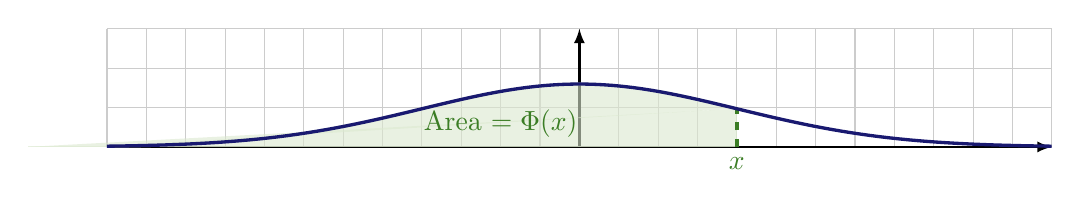
\begin{tikzpicture}[scale=2]
            \draw[thin,gray!40, step=0.25] (-3,0) grid (3, 0.75);
            \draw[thick, ->, >=latex] (-3,0)--(3,0);
            \draw[thick, ->, >=latex] (0,0)--(0,0.75);
    
            \def\sd{1};
            \def\mean{0};
            \def\r{1}

            \coordinate (CurveRightEdge) at (\r, {exp(-0.5*((\r-\mean)/\sd)^2)/sqrt(6.28*\sd)});
    
            \filldraw [OliveGreen!15, opacity=0.6, very thick, domain=-3:\r, samples=100] plot (\x,{exp(-0.5*((\x-\mean)/\sd)^2)/sqrt(6.28*\sd)});
            \filldraw [OliveGreen!15, opacity=0.6] (-3.5, 0) -- (\r, 0) -- (CurveRightEdge);
    
            \draw[OliveGreen, very thick, dashed] (\r, 0) node[below] {\(x\)} -- (CurveRightEdge);
    
            \draw [MidnightBlue, very thick, domain=-3:3, samples=100] plot (\x,{exp(-0.5*((\x-\mean)/\sd)^2)/sqrt(6.28*\sd)});

            \node[OliveGreen] at (-0.5, 0.15) {Area \(= \Phi(x)\)};
        \end{tikzpicture}
    \end{figure}

    \item \textbf{Table 5: Percentage points of the normal distribution.}
    
    \begin{itemize}
        \item Tabulates pairs of values \(P\) and \(x(P)\) satisfing the equation
        %
        \[\frac{P}{100} = \frac{1}{\sqrt{2\pi}} \int_{x(P)}^{\infty} e^{-\frac{1}{2}} \,dt\]
        %
        which can be graphically represented as the area under a standardised normal distribution curve to the right of some given vertical line.

        \item The percentage \(P/100\) gives the probability that a random variable with a \textit{standardised} normal distribution takes a value greater than or equal to \(x(P)\).
        
        \item This can be used to convert confidence levels to critical \(z\)-scores. For example, for a confidence level of \(95\%\), we set \(P/100 = (1 - 95\%)/2\) to get \(P = 2.5\). According to the table, this corresponds to \(x(P) = 1.96\).
    \end{itemize}

    
\end{itemize}